\documentclass[]{article}
\usepackage{lmodern}
\usepackage{amssymb,amsmath}
\usepackage{ifxetex,ifluatex}
\usepackage{fixltx2e} % provides \textsubscript
\ifnum 0\ifxetex 1\fi\ifluatex 1\fi=0 % if pdftex
  \usepackage[T1]{fontenc}
  \usepackage[utf8]{inputenc}
\else % if luatex or xelatex
  \ifxetex
    \usepackage{mathspec}
  \else
    \usepackage{fontspec}
  \fi
  \defaultfontfeatures{Ligatures=TeX,Scale=MatchLowercase}
\fi
% use upquote if available, for straight quotes in verbatim environments
\IfFileExists{upquote.sty}{\usepackage{upquote}}{}
% use microtype if available
\IfFileExists{microtype.sty}{%
\usepackage{microtype}
\UseMicrotypeSet[protrusion]{basicmath} % disable protrusion for tt fonts
}{}
\usepackage[margin=1in]{geometry}
\usepackage{hyperref}
\hypersetup{unicode=true,
            pdftitle={Narrative of original analysis},
            pdfauthor={Renata Diaz},
            pdfborder={0 0 0},
            breaklinks=true}
\urlstyle{same}  % don't use monospace font for urls
\usepackage{color}
\usepackage{fancyvrb}
\newcommand{\VerbBar}{|}
\newcommand{\VERB}{\Verb[commandchars=\\\{\}]}
\DefineVerbatimEnvironment{Highlighting}{Verbatim}{commandchars=\\\{\}}
% Add ',fontsize=\small' for more characters per line
\usepackage{framed}
\definecolor{shadecolor}{RGB}{248,248,248}
\newenvironment{Shaded}{\begin{snugshade}}{\end{snugshade}}
\newcommand{\KeywordTok}[1]{\textcolor[rgb]{0.13,0.29,0.53}{\textbf{#1}}}
\newcommand{\DataTypeTok}[1]{\textcolor[rgb]{0.13,0.29,0.53}{#1}}
\newcommand{\DecValTok}[1]{\textcolor[rgb]{0.00,0.00,0.81}{#1}}
\newcommand{\BaseNTok}[1]{\textcolor[rgb]{0.00,0.00,0.81}{#1}}
\newcommand{\FloatTok}[1]{\textcolor[rgb]{0.00,0.00,0.81}{#1}}
\newcommand{\ConstantTok}[1]{\textcolor[rgb]{0.00,0.00,0.00}{#1}}
\newcommand{\CharTok}[1]{\textcolor[rgb]{0.31,0.60,0.02}{#1}}
\newcommand{\SpecialCharTok}[1]{\textcolor[rgb]{0.00,0.00,0.00}{#1}}
\newcommand{\StringTok}[1]{\textcolor[rgb]{0.31,0.60,0.02}{#1}}
\newcommand{\VerbatimStringTok}[1]{\textcolor[rgb]{0.31,0.60,0.02}{#1}}
\newcommand{\SpecialStringTok}[1]{\textcolor[rgb]{0.31,0.60,0.02}{#1}}
\newcommand{\ImportTok}[1]{#1}
\newcommand{\CommentTok}[1]{\textcolor[rgb]{0.56,0.35,0.01}{\textit{#1}}}
\newcommand{\DocumentationTok}[1]{\textcolor[rgb]{0.56,0.35,0.01}{\textbf{\textit{#1}}}}
\newcommand{\AnnotationTok}[1]{\textcolor[rgb]{0.56,0.35,0.01}{\textbf{\textit{#1}}}}
\newcommand{\CommentVarTok}[1]{\textcolor[rgb]{0.56,0.35,0.01}{\textbf{\textit{#1}}}}
\newcommand{\OtherTok}[1]{\textcolor[rgb]{0.56,0.35,0.01}{#1}}
\newcommand{\FunctionTok}[1]{\textcolor[rgb]{0.00,0.00,0.00}{#1}}
\newcommand{\VariableTok}[1]{\textcolor[rgb]{0.00,0.00,0.00}{#1}}
\newcommand{\ControlFlowTok}[1]{\textcolor[rgb]{0.13,0.29,0.53}{\textbf{#1}}}
\newcommand{\OperatorTok}[1]{\textcolor[rgb]{0.81,0.36,0.00}{\textbf{#1}}}
\newcommand{\BuiltInTok}[1]{#1}
\newcommand{\ExtensionTok}[1]{#1}
\newcommand{\PreprocessorTok}[1]{\textcolor[rgb]{0.56,0.35,0.01}{\textit{#1}}}
\newcommand{\AttributeTok}[1]{\textcolor[rgb]{0.77,0.63,0.00}{#1}}
\newcommand{\RegionMarkerTok}[1]{#1}
\newcommand{\InformationTok}[1]{\textcolor[rgb]{0.56,0.35,0.01}{\textbf{\textit{#1}}}}
\newcommand{\WarningTok}[1]{\textcolor[rgb]{0.56,0.35,0.01}{\textbf{\textit{#1}}}}
\newcommand{\AlertTok}[1]{\textcolor[rgb]{0.94,0.16,0.16}{#1}}
\newcommand{\ErrorTok}[1]{\textcolor[rgb]{0.64,0.00,0.00}{\textbf{#1}}}
\newcommand{\NormalTok}[1]{#1}
\usepackage{graphicx,grffile}
\makeatletter
\def\maxwidth{\ifdim\Gin@nat@width>\linewidth\linewidth\else\Gin@nat@width\fi}
\def\maxheight{\ifdim\Gin@nat@height>\textheight\textheight\else\Gin@nat@height\fi}
\makeatother
% Scale images if necessary, so that they will not overflow the page
% margins by default, and it is still possible to overwrite the defaults
% using explicit options in \includegraphics[width, height, ...]{}
\setkeys{Gin}{width=\maxwidth,height=\maxheight,keepaspectratio}
\usepackage[normalem]{ulem}
% avoid problems with \sout in headers with hyperref:
\pdfstringdefDisableCommands{\renewcommand{\sout}{}}
\IfFileExists{parskip.sty}{%
\usepackage{parskip}
}{% else
\setlength{\parindent}{0pt}
\setlength{\parskip}{6pt plus 2pt minus 1pt}
}
\setlength{\emergencystretch}{3em}  % prevent overfull lines
\providecommand{\tightlist}{%
  \setlength{\itemsep}{0pt}\setlength{\parskip}{0pt}}
\setcounter{secnumdepth}{0}
% Redefines (sub)paragraphs to behave more like sections
\ifx\paragraph\undefined\else
\let\oldparagraph\paragraph
\renewcommand{\paragraph}[1]{\oldparagraph{#1}\mbox{}}
\fi
\ifx\subparagraph\undefined\else
\let\oldsubparagraph\subparagraph
\renewcommand{\subparagraph}[1]{\oldsubparagraph{#1}\mbox{}}
\fi

%%% Use protect on footnotes to avoid problems with footnotes in titles
\let\rmarkdownfootnote\footnote%
\def\footnote{\protect\rmarkdownfootnote}

%%% Change title format to be more compact
\usepackage{titling}

% Create subtitle command for use in maketitle
\providecommand{\subtitle}[1]{
  \posttitle{
    \begin{center}\large#1\end{center}
    }
}

\setlength{\droptitle}{-2em}

  \title{Narrative of original analysis}
    \pretitle{\vspace{\droptitle}\centering\huge}
  \posttitle{\par}
    \author{Renata Diaz}
    \preauthor{\centering\large\emph}
  \postauthor{\par}
      \predate{\centering\large\emph}
  \postdate{\par}
    \date{5/14/2019}


\begin{document}
\maketitle

A walkthrough of Ernest (2005)'s original analytical approach, from
close reading of the paper.

\subsection{Questions}\label{questions}

\begin{enumerate}
\def\labelenumi{\arabic{enumi}.}
\tightlist
\item
  Is energy use across body size categories (regardless of species)
  uniform or multimodal?
\end{enumerate}

\begin{itemize}
\tightlist
\item
  uniform would correspond generally to energetic equivalence/Damuth's
  rule.
\item
  multimodal might suggest different resource availability for different
  body sizes.
\end{itemize}

\begin{enumerate}
\def\labelenumi{\arabic{enumi}.}
\setcounter{enumi}{1}
\tightlist
\item
  If energy use is not uniform across body size categories, does the
  species level body size distribution correspond to modes of energy
  use?
\end{enumerate}

\begin{itemize}
\tightlist
\item
  i.e.~are there more species with mean body sizes around the modes of
  the body size-energy use distribution?
\item
  if so, maybe it's good to be certain sizes, and species accumulate at
  those optima.
\end{itemize}

\subsection{Data}\label{data}

\paragraph{Ernest data}\label{ernest-data}

Ernest drew data from the Andrews LTER, the Sevilleta, Niwot Ridge, and
Portal.

The data available online do not quite match the descriptive statistics
reported in Ernest (2005).

\paragraph{\texorpdfstring{Translation to
\texttt{replicate-becs}}{Translation to replicate-becs}}\label{translation-to-replicate-becs}

Download raw data. By default data will be stored in subdirectories of
\texttt{replicate-becs/data/paper/raw/} for each site.

\begin{Shaded}
\begin{Highlighting}[]
\KeywordTok{download_raw_paper_data}\NormalTok{()}
\end{Highlighting}
\end{Shaded}

Process raw data into the appropriate format. This is a data table with
a record for each individual and columns for \texttt{species} and
\texttt{weight} in grams. By default these tables will be stored in
subdirectores of \texttt{replicate-becs/data/paper/processed}.

\begin{Shaded}
\begin{Highlighting}[]
\KeywordTok{process_raw_data}\NormalTok{()}
\end{Highlighting}
\end{Shaded}

\begin{verbatim}
## Loading in data version 1.106.0
\end{verbatim}

\begin{verbatim}
## [1] TRUE
\end{verbatim}

Load data tables for each community. There should be 9 communities.

\begin{Shaded}
\begin{Highlighting}[]
\NormalTok{communities <-}\StringTok{ }\KeywordTok{load_paper_data}\NormalTok{()}

\KeywordTok{length}\NormalTok{(communities)}
\end{Highlighting}
\end{Shaded}

\begin{verbatim}
## [1] 9
\end{verbatim}

Each community should be a data table with columns for species and size
for each individual, for example:

\begin{Shaded}
\begin{Highlighting}[]
\KeywordTok{names}\NormalTok{(communities)}
\end{Highlighting}
\end{Shaded}

\begin{verbatim}
## [1] "andrews"      "niwot"        "portal"       "sev-5pgrass" 
## [5] "sev-5plarrea" "sev-goatdraw" "sev-rsgrass"  "sev-rslarrea"
## [9] "sev-two22"
\end{verbatim}

\begin{Shaded}
\begin{Highlighting}[]
\KeywordTok{head}\NormalTok{(communities[[}\DecValTok{1}\NormalTok{]])}
\end{Highlighting}
\end{Shaded}

\begin{verbatim}
##   individual_species_ids individual_sizes
## 1                   SOTR              4.0
## 2                   PEMA             16.5
## 3                   GLSA            167.0
## 4                   MIOR             13.0
## 5                   PEMA             14.0
## 6                   GLSA            142.0
\end{verbatim}

\subsection{Constructing
distributions/metrics}\label{constructing-distributionsmetrics}

\subsubsection{Body size-energy use distributions
(BSED)}\label{body-size-energy-use-distributions-bsed}

\paragraph{Ernest method}\label{ernest-method}

\begin{itemize}
\tightlist
\item
  Per individual, calculate metabolic rate as metabolic rate
  \(B \propto M^\frac{3}{4}\) where \(M\) is mass in grams.
\item
  Sum energy use of all individuals in body size classes of .2 natural
  log units.
\item
  Also try classes of .1 and .3 natural log units
\item
  Convert raw energy use values for each body size class into the
  proportion of all the energy used in that community used by that body
  size class. This allows for comparisons between communities.
\end{itemize}

\begin{figure}
\centering
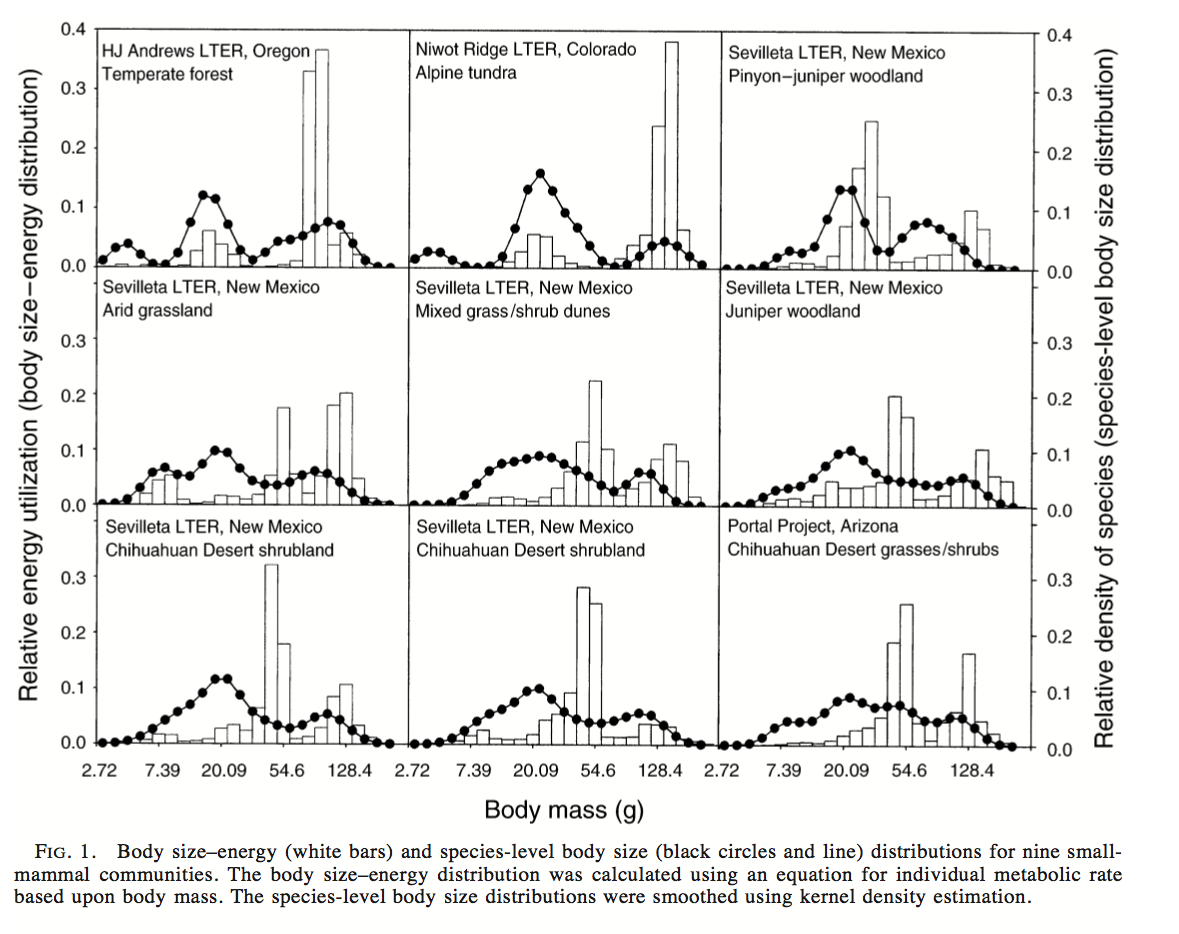
\includegraphics{../ernest-2005-files/ernest2005_fig1.png}
\caption{Ernest 2005 Fig 1}
\end{figure}

\paragraph{\texorpdfstring{Translation to
\texttt{replicate-becs}}{Translation to replicate-becs}}\label{translation-to-replicate-becs-1}

For every individual, calculate metabolic rate and assign to a size
class.

\begin{Shaded}
\begin{Highlighting}[]
\NormalTok{communities_energy <-}\StringTok{ }\KeywordTok{lapply}\NormalTok{(communities, }\DataTypeTok{FUN =}\NormalTok{ make_community_table, }\DataTypeTok{ln_units =} \FloatTok{0.2}\NormalTok{)}

\KeywordTok{head}\NormalTok{(communities_energy[[}\DecValTok{1}\NormalTok{]])}
\end{Highlighting}
\end{Shaded}

\begin{verbatim}
##   individual_species_ids individual_sizes individual_energy size_class
## 1                   SOTR              4.0          2.828427        1.2
## 2                   PEMA             16.5          8.186777        2.8
## 3                   GLSA            167.0         46.455523        5.0
## 4                   MIOR             13.0          6.846325        2.4
## 5                   PEMA             14.0          7.237624        2.6
## 6                   GLSA            142.0         41.135451        4.8
##   size_class_g
## 1     3.320117
## 2    16.444647
## 3   148.413159
## 4    11.023176
## 5    13.463738
## 6   121.510418
\end{verbatim}

For each community, sum total energy use for each size class, and
convert to the proportion of total energy use for that community.

\begin{Shaded}
\begin{Highlighting}[]
\NormalTok{bseds <-}\StringTok{ }\KeywordTok{lapply}\NormalTok{(communities_energy, }\DataTypeTok{FUN =}\NormalTok{ make_bsed)}

\KeywordTok{head}\NormalTok{(bseds[[}\DecValTok{1}\NormalTok{]])}
\end{Highlighting}
\end{Shaded}

\begin{verbatim}
## # A tibble: 6 x 4
##   size_class size_class_g total_energy total_energy_proportional
##        <dbl>        <dbl>        <dbl>                     <dbl>
## 1        0.6         1.82         1.68                  0.000211
## 2        1           2.72        20.6                   0.00259 
## 3        1.2         3.32       239.                    0.0301  
## 4        1.4         4.06        49.4                   0.00621 
## 5        1.6         4.95       195.                    0.0246  
## 6        1.8         6.05        21.1                   0.00265
\end{verbatim}

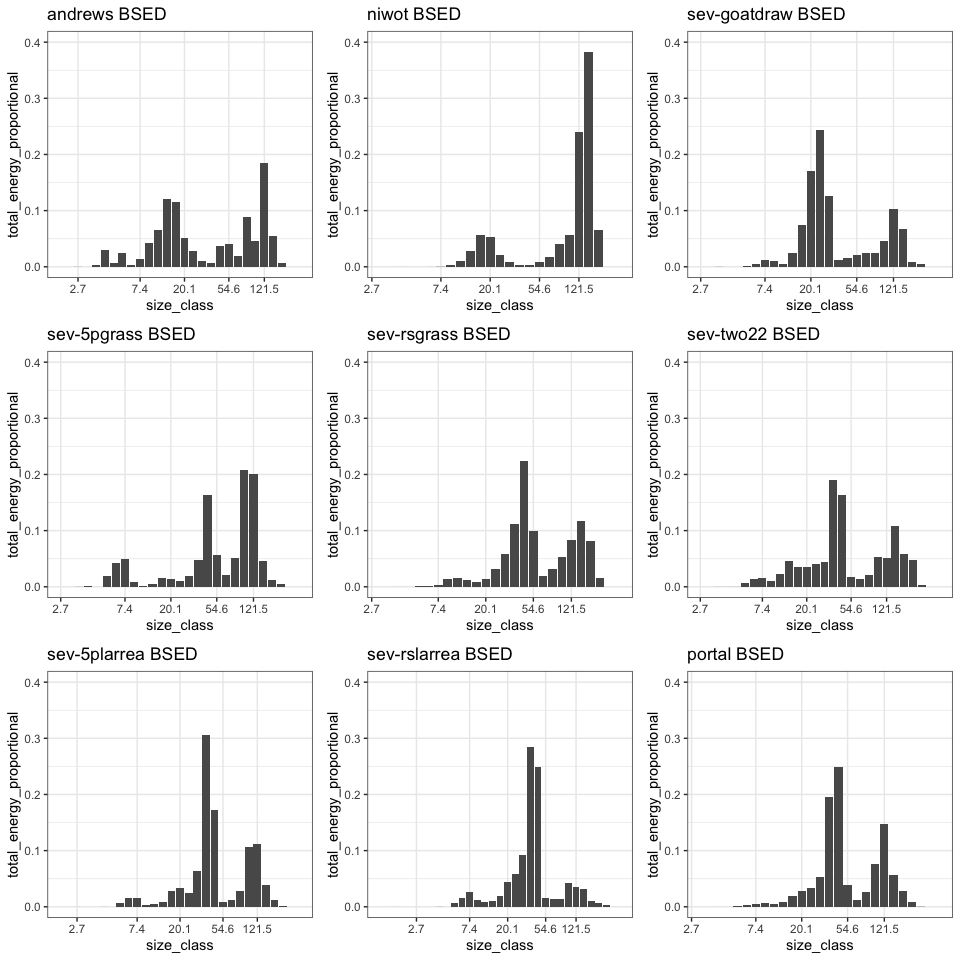
\includegraphics{ernest2005_replication_files/figure-latex/plot bseds-1.pdf}

\subsubsection{Species-level body size distributions
(BSD)}\label{species-level-body-size-distributions-bsd}

\paragraph{Ernest method}\label{ernest-method-1}

\begin{itemize}
\tightlist
\item
  Frequency distributions of mean mass of each species in a community.
\item
  For plotting (but not statistics), smoothed using kernel density
  estimation.
\item
  Gaussian kernel to mimic the actual body size distribution in log
  space
\item
  avg. std dev of the mean of the logged masses = smoothing parameter
  \(h\)
\item
  align sampling points with the midpoint of each size class in the BSED
\item
  after Manly 1996, ``Are there clumps in body-size distributions?'',
  \emph{Ecology}
\end{itemize}

\paragraph{\texorpdfstring{Translation to
\texttt{replicate-becs}}{Translation to replicate-becs}}\label{translation-to-replicate-becs-2}

Calculate mean mass of each species in each community.

\begin{Shaded}
\begin{Highlighting}[]
\NormalTok{bsds <-}\StringTok{ }\KeywordTok{lapply}\NormalTok{(communities, }\DataTypeTok{FUN =}\NormalTok{ make_bsd) }

\KeywordTok{head}\NormalTok{(bsds[[}\DecValTok{1}\NormalTok{]])}
\end{Highlighting}
\end{Shaded}

\begin{verbatim}
## # A tibble: 6 x 6
##   individual_specie~ species_mean_ma~ ln_mass size_class size_class_g stdev
##   <chr>                         <dbl>   <dbl>      <dbl>        <dbl> <dbl>
## 1 CLCA                           17.9    2.88        2.8        16.4   1.19
## 2 GLSA                          117.     4.76        4.6        99.5   1.19
## 3 MIOR                           14.9    2.70        2.6        13.5   1.19
## 4 NEGI                            6.5    1.87        1.8         6.05  1.19
## 5 PEMA                           14.9    2.70        2.6        13.5   1.19
## 6 SCOR                           54.4    4.00        3.8        44.7   1.19
\end{verbatim}

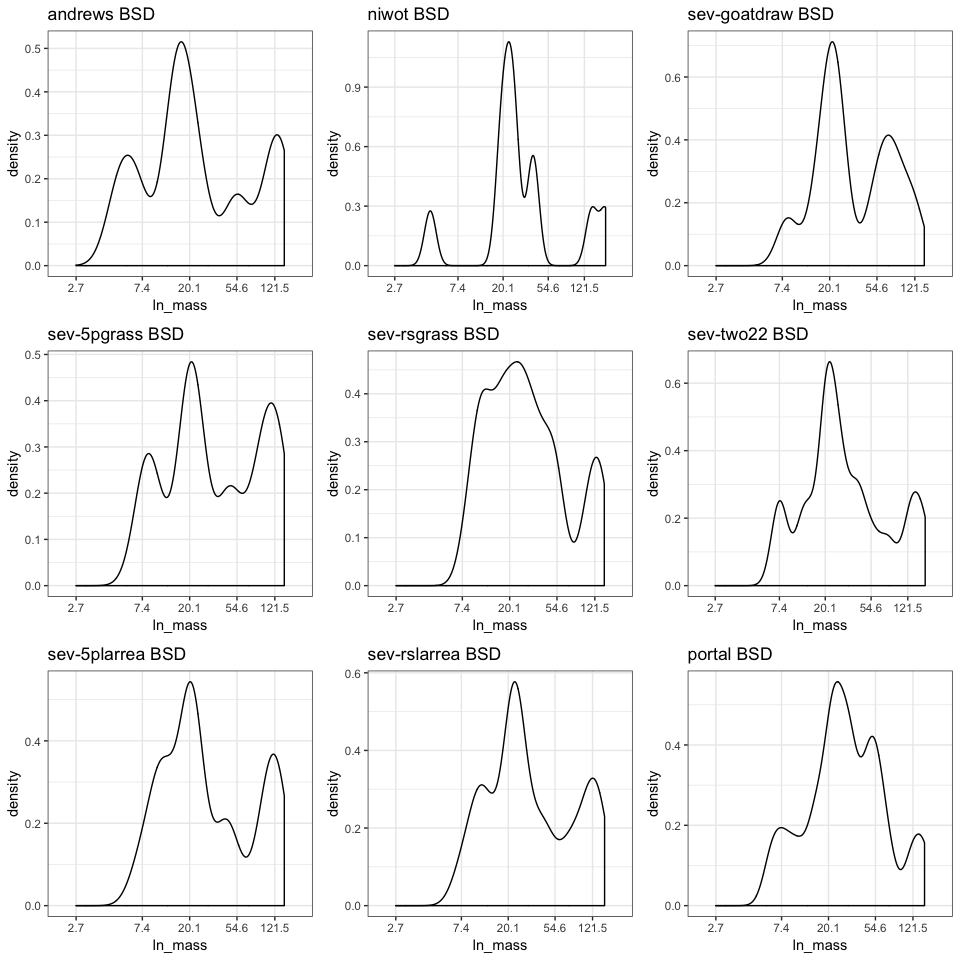
\includegraphics{ernest2005_replication_files/figure-latex/plot bsds-1.pdf}

\subsubsection{\texorpdfstring{Energetic dominance
(\(D_E\))}{Energetic dominance (D\_E)}}\label{energetic-dominance-d_e}

\begin{itemize}
\tightlist
\item
  Define ``energy use modes'' as contiguous body size classes where the
  energy use of each size class \textgreater{} 5\% of the community
  total.
\item
  i.e.~a little bit more than the expectation if energy use is uniform
  across all body sizes
\item
  RMD is unsure of this. Doesn't the uniform expectation depend on the
  number of size classes?
\item
  Calculate the total energy use for each species in the mode.
\item
  Calculate the ``dominance'' of the species with the highest energy use
  in that mode as \(D_E = p_{max}\), where \(p_{max}\) is the maximum
  proportion of energy use by any one species in a mode.
\item
  ``a modification of the Berger-Parker dominance index (Berger and
  Parker 1970)''
\end{itemize}

\paragraph{\texorpdfstring{Translation to
\texttt{replicate-becs}}{Translation to replicate-becs}}\label{translation-to-replicate-becs-3}

\begin{itemize}
\tightlist
\item
  Find contiguous size classes where each class has \textgreater{}5\% of
  total energy use
\item
  Calculate the total energy use for each species, and the proportion
  held by the species with the highest energy use (\(p_{max}\))
\item
  Return \(p_{max}\) for every mode, along with the min and max size
  classes in that mode for each community
\end{itemize}

\begin{Shaded}
\begin{Highlighting}[]
\NormalTok{energetic_dom <-}\StringTok{ }\KeywordTok{lapply}\NormalTok{(communities_energy, }\DataTypeTok{FUN =}\NormalTok{ energetic_dominance) }

\KeywordTok{head}\NormalTok{(energetic_dom[[}\DecValTok{1}\NormalTok{]])}
\end{Highlighting}
\end{Shaded}

\begin{verbatim}
## # A tibble: 3 x 4
##   mode_id e_dominance size_class_min size_class_max
##     <dbl>       <dbl>          <dbl>          <dbl>
## 1       1       0.766            2.4            3  
## 2       2       1                4.4            4.4
## 3       3       0.979            4.8            5
\end{verbatim}

\begin{itemize}
\tightlist
\item
  To plot, combine all modes from all communities and plot a histogram
  of \(D_E\) values.
\end{itemize}

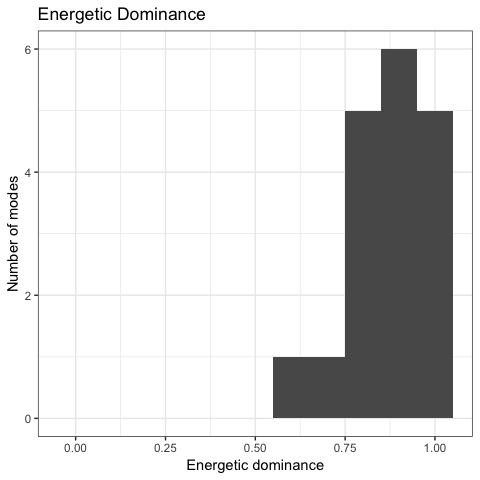
\includegraphics{ernest2005_replication_files/figure-latex/plot Ed-1.pdf}

\begin{itemize}
\tightlist
\item
  Out of curiousity, what happens if we define the modes with the cutoff
  proportional to the number of size classes (instead of a fixed 5\%?)
\end{itemize}

\begin{Shaded}
\begin{Highlighting}[]
\NormalTok{energetic_dom_prop <-}\StringTok{ }\KeywordTok{lapply}\NormalTok{(communities_energy, }\DataTypeTok{FUN =}\NormalTok{ energetic_dominance, }\DataTypeTok{mode_cutoff =} \StringTok{'prop'}\NormalTok{) }
\end{Highlighting}
\end{Shaded}

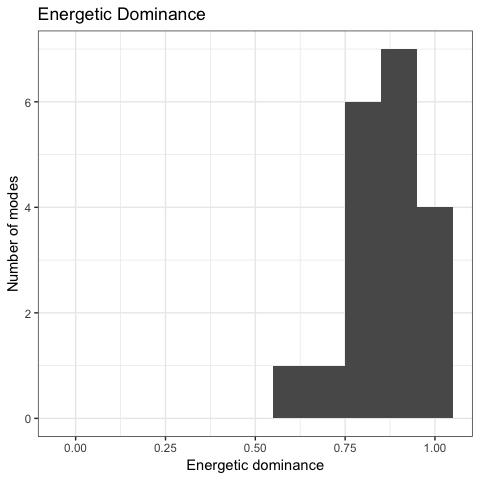
\includegraphics{ernest2005_replication_files/figure-latex/plot edom proportional-1.pdf}

\begin{itemize}
\tightlist
\item
  RMD: They're similar.
\end{itemize}

\subsection{Statistical tests}\label{statistical-tests}

\subsubsection{Comparing BSEDs to
uniform}\label{comparing-bseds-to-uniform}

\paragraph{Ernest approach}\label{ernest-approach}

\begin{itemize}
\tightlist
\item
  Use bootstrap sampling to compare to uniform distributions.
\item
  For every community, draw 10000 samples (sim communities):
\item
  Same number of individuals as the empirical community, drawn from a
  uniform distribution ranging from the smallest to largest \sout{body
  size} individual metabolic rate of any individual in that community.
\item
  For sim communities and the empirical community, calculate a
  distribution overlap index (\(DOI\)):
\item
  \(DOI = \sum_k {|y_{ak} - y_{bk}|}\) where \(y\) is the value for size
  class \(k\) in communities \(a\) and \(b\).
\item
  \(DOI\) values will range from 0 (complete overlap) to 2 (no overlap).
\item
  For the BSED bootstraps, community \(a\) is the empirical or sim
  distribution, and community \(b\) is a true uniform distribution
  \sout{(i.e. \(y_{bk} = \frac{1}{\max(k)}\) for all \(k\))}
\item
  ``True uniform distribution'': There are exactly the same number of
  individuals of every size.
\item
  Calculate the \(DOI\) for all sim communities and the empirical.
\item
  Find the quantile value for the empirical \(DOI\) compared to the
  distribution of sim \(DOI\)s. This is the p-value; i.e.~the proportion
  of sim uniform distributions with DOIs greater than the empirical.
\end{itemize}

\paragraph{\texorpdfstring{Translation to
\texttt{replicate-becs}}{Translation to replicate-becs}}\label{translation-to-replicate-becs-4}

\begin{itemize}
\tightlist
\item
  For a given empirical community, draw 10000 sim communities each with
  the same number of individuals \(n\), with body sizes randomly drawn
  from a uniform distribution from the minimum to maximum body size in
  that community.
\item
  Calculate the \(DOI\) of each sim community compared to a true uniform
  distribution.
\item
  True uniform distribution = every size from the minimum to the maximum
  size in the community (by .1g) has exactly one individual.
\end{itemize}

\begin{Shaded}
\begin{Highlighting}[]
\NormalTok{bsed_uniform_bootstraps <-}\StringTok{ }\KeywordTok{lapply}\NormalTok{(communities, }\DataTypeTok{FUN =}\NormalTok{ community_bootstrap,  }\DataTypeTok{bootstrap_function =} \StringTok{'bootstrap_unif_bsed_doi'}\NormalTok{, }\DataTypeTok{nbootstraps =} \DecValTok{10}\NormalTok{)}
\end{Highlighting}
\end{Shaded}

\emph{See issue \#4 on github.}

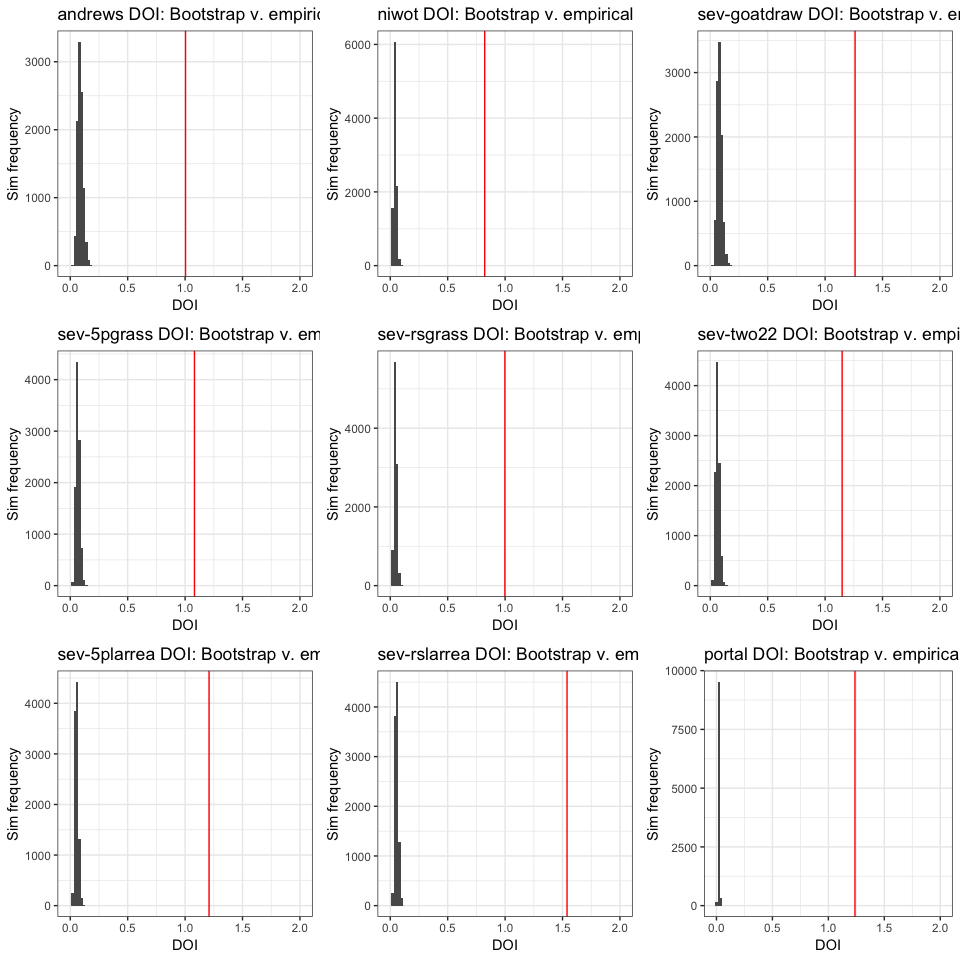
\includegraphics{ernest2005_replication_files/figure-latex/plot BSED-uniform bootstrap DOIs v empirical-1.pdf}

\subsubsection{Compare BSEDs among
communities}\label{compare-bseds-among-communities}

\paragraph{Ernest approach}\label{ernest-approach-1}

\begin{itemize}
\tightlist
\item
  For every pair of communities, create a pool of masses of all
  individuals from both communities.
\item
  Draw two new communities with the same number of individuals as the
  empirical communities, pulling masses at random from the pool, with
  replacement.
\item
  Calculate the DOI for the BSEDs of the two sample communities.
\item
  Repeat 10000 for each pair.
\item
  The P value is the proportion of sample DOIs greater (i.e.~less
  overlap) than the empirical value.
\end{itemize}

\paragraph{\texorpdfstring{Translation to
\texttt{replicate-becs}}{Translation to replicate-becs}}\label{translation-to-replicate-becs-5}

\begin{itemize}
\tightlist
\item
  For every pair of communities, pool all the masses
\item
  Resample two communities of the right sizes
\item
  Construct BSEDs for both communities
\item
  Calculate the DOI of the two BSEDs
\item
  Repeat 10000x
\end{itemize}

\begin{Shaded}
\begin{Highlighting}[]
\NormalTok{community_combination_indices =}\StringTok{ }\NormalTok{utils}\OperatorTok{::}\KeywordTok{combn}\NormalTok{(}\DataTypeTok{x =} \KeywordTok{c}\NormalTok{(}\DecValTok{1}\OperatorTok{:}\DecValTok{9}\NormalTok{), }\DataTypeTok{m =} \DecValTok{2}\NormalTok{, }\DataTypeTok{simplify =} \OtherTok{TRUE}\NormalTok{) }\OperatorTok
\StringTok{  }\KeywordTok{t}\NormalTok{() }\OperatorTok
\StringTok{  }\KeywordTok{as.data.frame}\NormalTok{() }\OperatorTok
\StringTok{  }\NormalTok{dplyr}\OperatorTok{::}\KeywordTok{rename}\NormalTok{(}\DataTypeTok{community_a =}\NormalTok{ V1, }\DataTypeTok{community_b =}\NormalTok{ V2)}

\NormalTok{combine_communities =}\StringTok{ }\ControlFlowTok{function}\NormalTok{(indices, communities) \{}
\NormalTok{  community_combination =}\StringTok{ }\KeywordTok{list}\NormalTok{(}\DataTypeTok{community_a =}\NormalTok{ communities[[indices[}\DecValTok{1}\NormalTok{]]], }\DataTypeTok{community_b =}\NormalTok{ communities[[indices[}\DecValTok{2}\NormalTok{]]], }\DataTypeTok{community_names =} \KeywordTok{c}\NormalTok{(}\KeywordTok{names}\NormalTok{(communities)[[indices[}\DecValTok{1}\NormalTok{]]], }\KeywordTok{names}\NormalTok{(communities)[[indices[}\DecValTok{2}\NormalTok{]]]))}
  
  \KeywordTok{return}\NormalTok{(community_combination)}
\NormalTok{\}}

\NormalTok{community_combinations =}\StringTok{ }\KeywordTok{apply}\NormalTok{(community_combination_indices, }\DataTypeTok{MARGIN =} \DecValTok{1}\NormalTok{, }\DataTypeTok{FUN =}\NormalTok{ combine_communities, }\DataTypeTok{communities =}\NormalTok{ communities)}
\end{Highlighting}
\end{Shaded}

\begin{Shaded}
\begin{Highlighting}[]
\NormalTok{bsed_crosscomm_bootstraps =}\StringTok{ }\KeywordTok{lapply}\NormalTok{(community_combinations, }\DataTypeTok{FUN =}\NormalTok{ community_bootstrap, }
                                   \DataTypeTok{bootstrap_function =} \StringTok{'bootstrap_crosscomm_bseds'}\NormalTok{, }\DataTypeTok{nbootstraps =} \DecValTok{10}\NormalTok{)}
\end{Highlighting}
\end{Shaded}

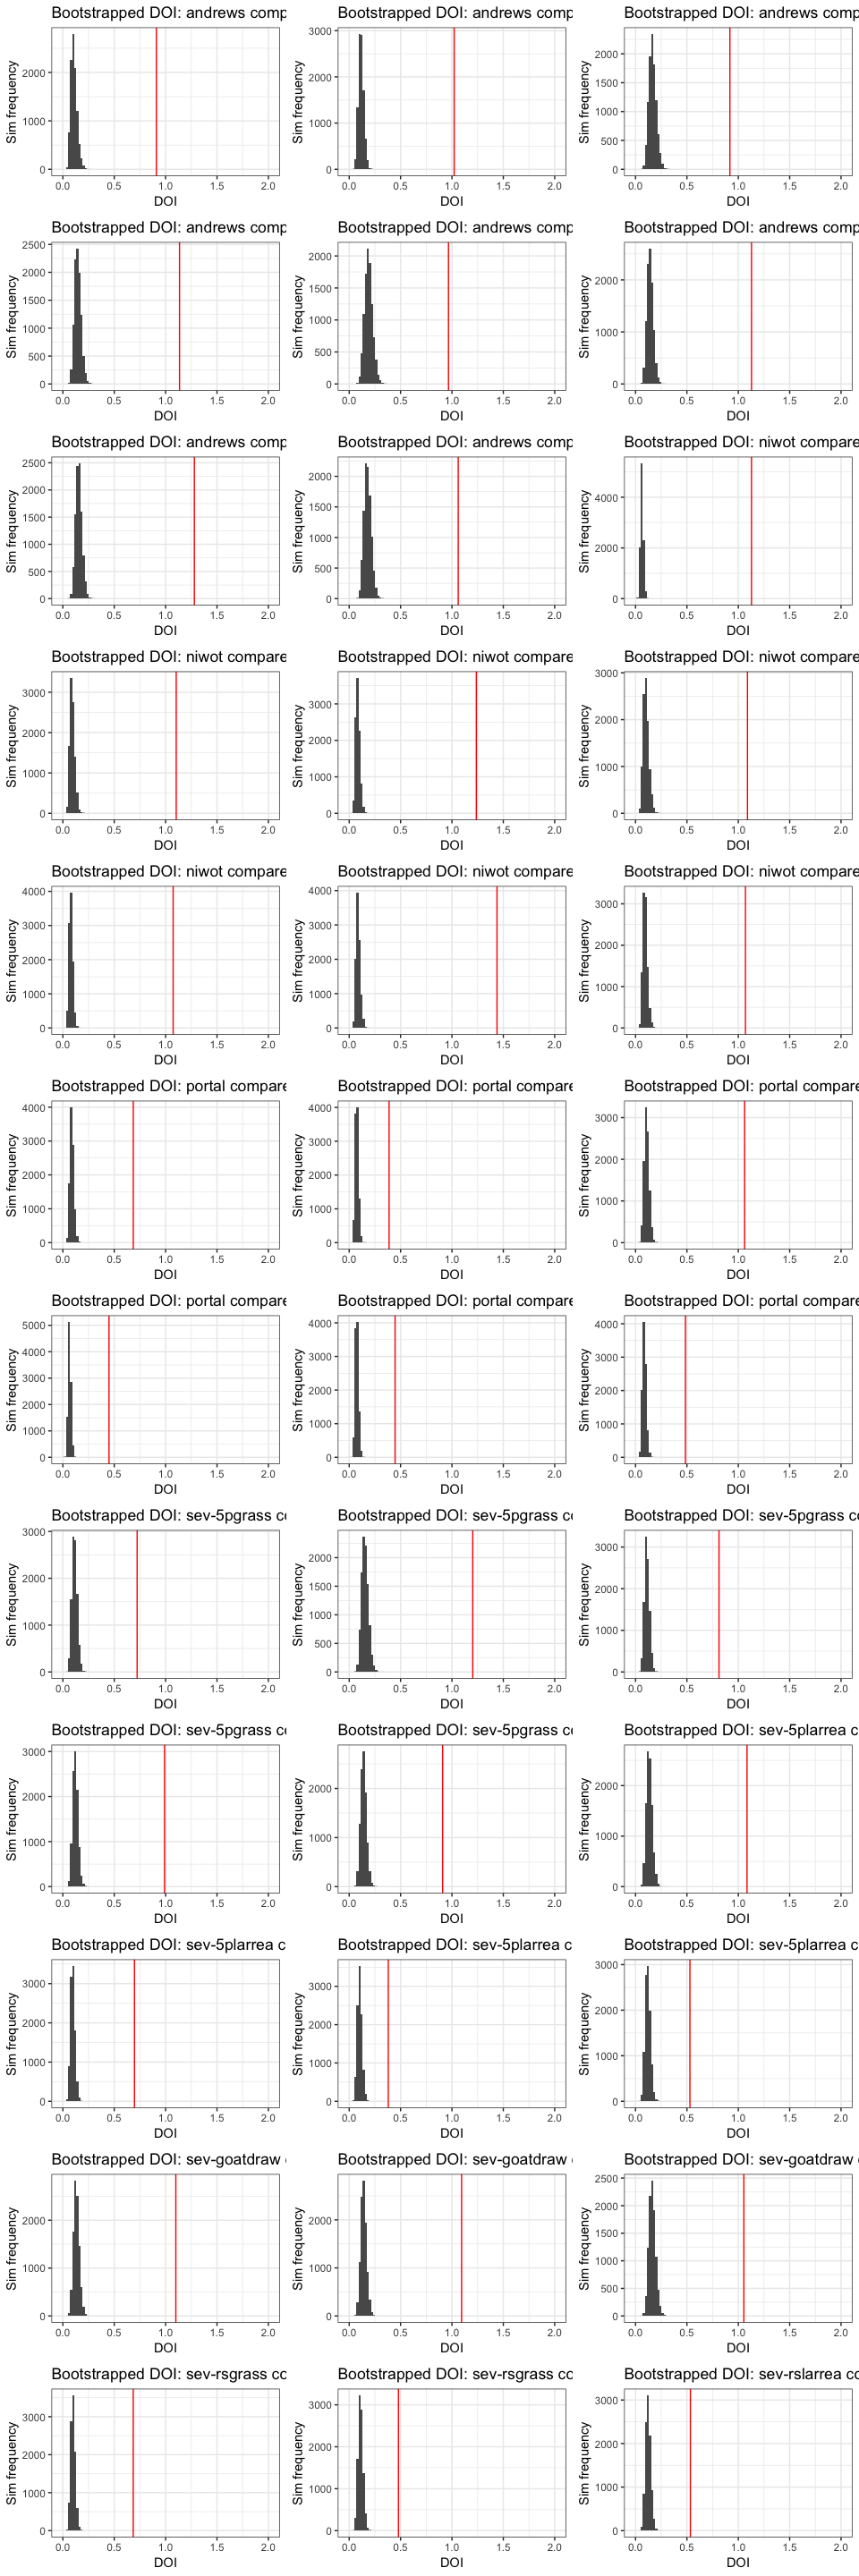
\includegraphics{ernest2005_replication_files/figure-latex/plot cross community comparisons-1.pdf}

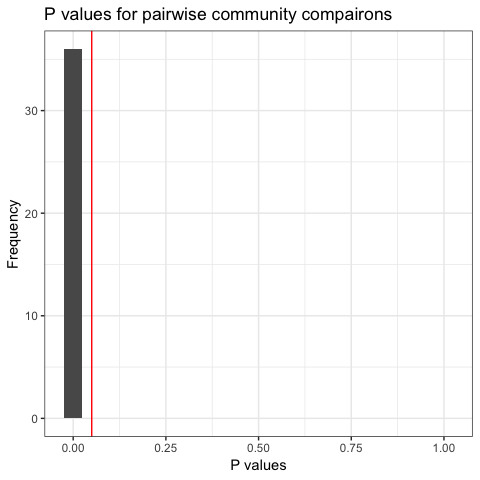
\includegraphics{ernest2005_replication_files/figure-latex/plot cross community p values-1.pdf}

See histogram of p values for comparisons to see if commuities' BSEDs
are the same or different.

\subsubsection{Testing BSDs for
uniformity}\label{testing-bsds-for-uniformity}

\paragraph{Matching communities}\label{matching-communities}

Ernest (2005) refers to the communities with the \texttt{site} column
above. To compare the communities above to the communities in the
resurrected data set, we can try to match them based on the BSD and BSED
plots (above) and species richness.

\begin{Shaded}
\begin{Highlighting}[]
\NormalTok{ernest_richness =}\StringTok{ }\KeywordTok{read.csv}\NormalTok{(here}\OperatorTok{::}\KeywordTok{here}\NormalTok{(}\StringTok{"ernest-2005-files/ernest_richness.csv"}\NormalTok{), }\DataTypeTok{stringsAsFactors =}\NormalTok{ F)}

\CommentTok{# Guesses based on body size plots}
\NormalTok{ernest_richness}\OperatorTok{$}\NormalTok{community_name <-}\StringTok{ }\KeywordTok{c}\NormalTok{(}\StringTok{'andrews'}\NormalTok{, }\StringTok{'niwot'}\NormalTok{, }\StringTok{'portal'}\NormalTok{, }\StringTok{'sev-5pgrass'}\NormalTok{, }
                                    \StringTok{'sev-rsgrass'}\NormalTok{, }\StringTok{'sev-two22'}\NormalTok{, }\StringTok{'sev-goatdraw'}\NormalTok{, }
                                    \StringTok{'sev-5plarrea'}\NormalTok{, }\StringTok{'sev-rslarrea'}\NormalTok{)}


\NormalTok{bsds_richness =}\StringTok{ }\KeywordTok{data.frame}\NormalTok{(}\DataTypeTok{community_name =} \KeywordTok{names}\NormalTok{(bsds), }\DataTypeTok{stringsAsFactors =}\NormalTok{ F)}
\NormalTok{bsds_richness}\OperatorTok{$}\NormalTok{new_richness =}\StringTok{ }\OtherTok{NA}
\ControlFlowTok{for}\NormalTok{(i }\ControlFlowTok{in} \DecValTok{1}\OperatorTok{:}\KeywordTok{nrow}\NormalTok{(bsds_richness))\{}
\NormalTok{  bsds_richness}\OperatorTok{$}\NormalTok{new_richness[i] =}\StringTok{ }\KeywordTok{nrow}\NormalTok{(bsds[[i]])}
\NormalTok{\}}

\CommentTok{# See if the richness values match}
\NormalTok{ernest_richness =}\StringTok{ }\NormalTok{ernest_richness }\OperatorTok
\StringTok{  }\NormalTok{dplyr}\OperatorTok{::}\KeywordTok{left_join}\NormalTok{(bsds_richness, }\DataTypeTok{by =} \StringTok{'community_name'}\NormalTok{) }\OperatorTok
\StringTok{  }\NormalTok{dplyr}\OperatorTok{::}\KeywordTok{mutate}\NormalTok{(}\DataTypeTok{richness_match =}\NormalTok{ (richness }\OperatorTok{==}\StringTok{ }\NormalTok{new_richness))}

\KeywordTok{print}\NormalTok{(ernest_richness)}
\end{Highlighting}
\end{Shaded}

\begin{verbatim}
##                 site richness community_name new_richness richness_match
## 1            andrews        9        andrews            9           TRUE
## 2              niwot       11          niwot           11           TRUE
## 3             portal       21         portal           19          FALSE
## 4          sev grass       18    sev-5pgrass           15          FALSE
## 5    sev grass shrub       20    sev-rsgrass           18          FALSE
## 6        sev juniper       21      sev-two22           18          FALSE
## 7 sev pinyon juniper       12   sev-goatdraw           12           TRUE
## 8          sev shrub       18   sev-5plarrea           15          FALSE
## 9        sev shrub 2       20   sev-rslarrea           20           TRUE
\end{verbatim}

We can get 2 (of 7) communities at the Sevilleta to match up, and Niwot
and Andrews. The other pairings are as close as possible.

Moving forward, we can compare the results of the Kolmogorov-Smirnov
tests based on the values in the appendix and these name pairings.

\begin{Shaded}
\begin{Highlighting}[]
\NormalTok{ernest_key =}\StringTok{ }\NormalTok{ernest_richness }\OperatorTok
\StringTok{  }\NormalTok{dplyr}\OperatorTok{::}\KeywordTok{select}\NormalTok{(site, community_name)}

\KeywordTok{write.csv}\NormalTok{(ernest_key, }\DataTypeTok{file =}\NormalTok{ here}\OperatorTok{::}\KeywordTok{here}\NormalTok{(}\StringTok{'ernest-2005-files/ernest_key.csv'}\NormalTok{), }\DataTypeTok{row.names =}\NormalTok{ F)}
\end{Highlighting}
\end{Shaded}

\paragraph{Ernest approach}\label{ernest-approach-2}

\begin{itemize}
\tightlist
\item
  \(\delta\)-corrected Kolmogorov-Smirnov test.
\item
  ``The \(\delta\)-corrected K-S test increases the power of the test
  when sample sizes are small (n \textless{} 25; Zar 1999)''
\item
  The \(\delta\)-corrected test is not widely discussed online.
\end{itemize}

\begin{Shaded}
\begin{Highlighting}[]
\NormalTok{ernest_bsds_uniform_results =}\StringTok{ }\KeywordTok{read.csv}\NormalTok{(here}\OperatorTok{::}\KeywordTok{here}\NormalTok{(}\StringTok{'ernest-2005-files/ernest_appendixA.csv'}\NormalTok{), }\DataTypeTok{stringsAsFactors =}\NormalTok{ F) }\OperatorTok
\StringTok{  }\NormalTok{dplyr}\OperatorTok{::}\KeywordTok{left_join}\NormalTok{(ernest_key, }\DataTypeTok{by =} \StringTok{'site'}\NormalTok{)}
\KeywordTok{print}\NormalTok{(ernest_bsds_uniform_results)}
\end{Highlighting}
\end{Shaded}

\begin{verbatim}
##                 site sample.size     d delta p_min p_max signif
## 1            andrews           9 0.210     1   0.5   1.0  FALSE
## 2              niwot          11 0.290     1   0.1   0.2  FALSE
## 3             portal          21 0.090     1   0.5   1.0  FALSE
## 4          sev grass          18 0.175     0   0.2   0.5  FALSE
## 5    sev grass shrub          20 0.102     0   0.5   1.0  FALSE
## 6        sev juniper          21 0.115     0   0.5   1.0  FALSE
## 7 sev pinyon juniper          12 0.120     0   0.5   1.0  FALSE
## 8          sev shrub          18 0.189     0   0.2   0.5  FALSE
## 9        sev shrub 2          20 0.137     0   0.5   1.0  FALSE
##   community_name
## 1        andrews
## 2          niwot
## 3         portal
## 4    sev-5pgrass
## 5    sev-rsgrass
## 6      sev-two22
## 7   sev-goatdraw
## 8   sev-5plarrea
## 9   sev-rslarrea
\end{verbatim}

\paragraph{\texorpdfstring{Translation to
\texttt{replicate-becs}:}{Translation to replicate-becs:}}\label{translation-to-replicate-becs-6}

\emph{From Zar (1999) \emph{Biostatistical Analysis}.}

\subparagraph{Base K-S test}\label{base-k-s-test}

\begin{itemize}
\tightlist
\item
  Take vector of measurements \(X_i\).
\item
  For each \(X_i\) record the observed frequency \(f_i\) (number of
  observations with that value).
\item
  Determine cumulative observed frequencies \(F_i\) and cumulative
  relative frequencies \(\textrm{rel}F_i\):
\item
  \(\textrm{rel}F_i = \frac{F_i}{n}\) where \(n\) is the number of
  measurements taken.
\item
  \(\textrm{rel}F_i\) is the proportion of the sample that is
  measurements \(\leq X_i\).
\item
  For each \(X_i\), determine the cumulative \emph{relative} expected
  frequency from the comparison distribution, \(\textrm{rel}\hat{F_i}\).
\item
  For a uniform distribution,
  \(\textrm{rel}\hat{F_i} = \frac{X_i - \min(X)}{\max(X) - \min(X)}\)
\item
  Determine \(D_i\) and \(D'_i\) as:
\item
  \(D_i = |{\textrm{rel}F_i - \textrm{rel}\hat{F_i}}|\)
\item
  \(D'_i = |{\textrm{rel}F_{i-1} - \textrm{rel}\hat{F_i}}|\)
\item
  note \(F_0 = 0\) so \(D'_1 = \textrm{rel}\hat{F_i}\)
\item
  The test statistic \(D\) is:
\item
  \(D = \max[(\max(D_i), (\max(D'_i)]\)
\item
  Compare to critical values from appendix.
\end{itemize}

\subparagraph{\texorpdfstring{\(\delta\)-corrected KS
test}{\textbackslash{}delta-corrected KS test}}\label{delta-corrected-ks-test}

\begin{itemize}
\tightlist
\item
  For small sample sizes (\textless{}25) we can obtain increased power
  using the \(\delta\)-corrected KS test.
\item
  For each \(i\) determine
\item
  \(\textrm{rel}G_i = \frac{F_i}{n + 1}\)
\item
  \(\textrm{rel}G'_i = \frac{F_i - 1}{n - 1}\)
\item
  Then obtain similar \(D\)s
\item
  \(D_{0, i} = |\textrm{rel}G_i - \textrm{rel}\hat{F_i}|\)
\item
  \(D_{1, i} = |\textrm{rel}G'_i - \textrm{rel}\hat{F_i}|\)
\item
  The test statistic is either \(\max(D_{0, i})\) or \(\max(D_{1, i})\),
  whichever leads to the highest level of significance/smallest
  probability. Look up significance in table from appendix. The 1 and 0
  are the \(\delta\)s.
\end{itemize}

Tables of critical values were entered by hand from the appendix to Zar
(1999).

\begin{verbatim}
##   community_name signif.x p_max.x p_min.x d_statistic               site
## 1        andrews     TRUE    0.02       0   0.4824239            andrews
## 2          niwot     TRUE    0.02       0   0.6140682              niwot
## 3         portal     TRUE    0.02       0   0.4946621             portal
## 4    sev-5pgrass     TRUE    0.02       0   0.3893173          sev grass
## 5   sev-5plarrea     TRUE    0.02       0   0.4624160          sev shrub
## 6   sev-goatdraw     TRUE    0.02       0   0.3881576 sev pinyon juniper
## 7    sev-rsgrass     TRUE    0.02       0   0.4672033    sev grass shrub
## 8   sev-rslarrea     TRUE    0.02       0   0.4343417        sev shrub 2
## 9      sev-two22     TRUE    0.02       0   0.5084637        sev juniper
##   sample.size     d delta p_min.y p_max.y signif.y
## 1           9 0.210     1     0.5     1.0    FALSE
## 2          11 0.290     1     0.1     0.2    FALSE
## 3          21 0.090     1     0.5     1.0    FALSE
## 4          18 0.175     0     0.2     0.5    FALSE
## 5          18 0.189     0     0.2     0.5    FALSE
## 6          12 0.120     0     0.5     1.0    FALSE
## 7          20 0.102     0     0.5     1.0    FALSE
## 8          20 0.137     0     0.5     1.0    FALSE
## 9          21 0.115     0     0.5     1.0    FALSE
\end{verbatim}

The \(\delta\) corrected KS test does not correspond to the results from
Ernest when the species mean body size values are on an untransformed
scale.

Using the natural log of the species mean body size value,
however\ldots{}:

\begin{verbatim}
##   community_name signif.x p_max.x p_min.x d_statistic               site
## 1        andrews    FALSE     1.0     0.5   0.1398433            andrews
## 2          niwot    FALSE     0.5     0.1   0.2973462              niwot
## 3         portal    FALSE     1.0     0.5   0.1436705             portal
## 4    sev-5pgrass    FALSE     1.0     0.5   0.1252882          sev grass
## 5   sev-5plarrea    FALSE     0.5     0.1   0.2037134          sev shrub
## 6   sev-goatdraw    FALSE     1.0     0.5   0.1327084 sev pinyon juniper
## 7    sev-rsgrass    FALSE     1.0     0.5   0.1617653    sev grass shrub
## 8   sev-rslarrea    FALSE     1.0     0.5   0.1415647        sev shrub 2
## 9      sev-two22    FALSE     1.0     0.5   0.1663774        sev juniper
##   sample.size     d delta p_min.y p_max.y signif.y
## 1           9 0.210     1     0.5     1.0    FALSE
## 2          11 0.290     1     0.1     0.2    FALSE
## 3          21 0.090     1     0.5     1.0    FALSE
## 4          18 0.175     0     0.2     0.5    FALSE
## 5          18 0.189     0     0.2     0.5    FALSE
## 6          12 0.120     0     0.5     1.0    FALSE
## 7          20 0.102     0     0.5     1.0    FALSE
## 8          20 0.137     0     0.5     1.0    FALSE
## 9          21 0.115     0     0.5     1.0    FALSE
\end{verbatim}

With mean mass logged, all the results replicate qualitatively (i.e.~not
significantly different from uniform) and Niwot, for which the
currently-available data most closely matches that reported in Ernest
(2005), replicates almost exactly numerically.

\subsubsection{Comparing BSDs among
communities}\label{comparing-bsds-among-communities}

\paragraph{Ernest approach}\label{ernest-approach-3}

Ernest (2005) used a two-sample Kolmogorov-Smirnov test to compare every
possible combination of community-level BSDs.

\begin{verbatim}
##                site_a          site_b max_d ernest_p_val  community_a
## 1  sev pinyon juniper       sev grass 1.940        0.948 sev-goatdraw
## 2  sev pinyon juniper       sev shrub 0.222        0.869 sev-goatdraw
## 3           sev grass       sev shrub 0.167        0.964  sev-5pgrass
## 4  sev pinyon juniper     sev shrub 2 0.150        0.996 sev-goatdraw
## 5           sev grass     sev shrub 2 0.172        0.941  sev-5pgrass
## 6           sev shrub     sev shrub 2 0.161        0.967 sev-5plarrea
## 7  sev pinyon juniper sev grass shrub 0.150        0.996 sev-goatdraw
## 8           sev grass sev grass shrub 0.211        0.792  sev-5pgrass
## 9           sev shrub sev grass shrub 0.261        0.538 sev-5plarrea
## 10        sev shrub 2 sev grass shrub 0.150        0.978 sev-rslarrea
## 11 sev pinyon juniper     sev juniper 0.155        0.993 sev-goatdraw
## 12          sev grass     sev juniper 0.151        0.980  sev-5pgrass
## 13          sev shrub     sev juniper 0.183        0.903 sev-5plarrea
## 14        sev shrub 2     sev juniper 0.105        1.000 sev-rslarrea
## 15    sev grass shrub     sev juniper 0.112        1.000  sev-rsgrass
## 16 sev pinyon juniper          portal 0.155        0.993 sev-goatdraw
## 17          sev grass          portal 0.230        0.684  sev-5pgrass
## 18          sev shrub          portal 0.238        0.642 sev-5plarrea
## 19        sev shrub 2          portal 0.171        0.924 sev-rslarrea
## 20    sev grass shrub          portal 0.112        1.000  sev-rsgrass
## 21        sev juniper          portal 0.143        0.983    sev-two22
## 22 sev pinyon juniper           niwot 0.235        0.910 sev-goatdraw
## 23          sev grass           niwot 0.242        0.817  sev-5pgrass
## 24          sev shrub           niwot 0.227        0.872 sev-5plarrea
## 25        sev shrub 2           niwot 0.218        0.888 sev-rslarrea
## 26    sev grass shrub           niwot 0.259        0.727  sev-rsgrass
## 27        sev juniper           niwot 0.199        0.937    sev-two22
## 28             portal           niwot 0.247        0.772       portal
## 29 sev pinyon juniper         andrews 0.278        0.822 sev-goatdraw
## 30          sev grass         andrews 0.167        0.996  sev-5pgrass
## 31          sev shrub         andrews 0.222        0.928 sev-5plarrea
## 32        sev shrub 2         andrews 0.194        0.973 sev-rslarrea
## 33    sev grass shrub         andrews 0.206        0.956  sev-rsgrass
## 34        sev juniper         andrews 0.206        0.951    sev-two22
## 35             portal         andrews 0.206        0.951       portal
## 36              niwot         andrews 0.354        0.566        niwot
##     community_b
## 1   sev-5pgrass
## 2  sev-5plarrea
## 3  sev-5plarrea
## 4  sev-rslarrea
## 5  sev-rslarrea
## 6  sev-rslarrea
## 7   sev-rsgrass
## 8   sev-rsgrass
## 9   sev-rsgrass
## 10  sev-rsgrass
## 11    sev-two22
## 12    sev-two22
## 13    sev-two22
## 14    sev-two22
## 15    sev-two22
## 16       portal
## 17       portal
## 18       portal
## 19       portal
## 20       portal
## 21       portal
## 22        niwot
## 23        niwot
## 24        niwot
## 25        niwot
## 26        niwot
## 27        niwot
## 28        niwot
## 29      andrews
## 30      andrews
## 31      andrews
## 32      andrews
## 33      andrews
## 34      andrews
## 35      andrews
## 36      andrews
\end{verbatim}

\paragraph{\texorpdfstring{Translation to
\texttt{replicate-becs}}{Translation to replicate-becs}}\label{translation-to-replicate-becs-7}

\begin{Shaded}
\begin{Highlighting}[]
\CommentTok{# use same community combinations as before}

\NormalTok{bsd_crosscomm_ks =}\StringTok{ }\KeywordTok{lapply}\NormalTok{(community_combinations, }\DataTypeTok{FUN =}\NormalTok{ ks_bsd, }
                          \DataTypeTok{ln_mass_vals =}\NormalTok{ F)}
\end{Highlighting}
\end{Shaded}

\begin{verbatim}
##     community_b  community_a      ks_d   p_value             site_a
## 1       andrews        niwot 0.4646465 0.1651107              niwot
## 2       andrews       portal 0.2923977 0.5769685             portal
## 3       andrews  sev-5pgrass 0.3555556 0.3936294          sev grass
## 4       andrews sev-5plarrea 0.2888889 0.6408133          sev shrub
## 5       andrews sev-goatdraw 0.3888889 0.3445820 sev pinyon juniper
## 6       andrews  sev-rsgrass 0.2222222 0.9241602    sev grass shrub
## 7       andrews sev-rslarrea 0.3055556 0.4896041        sev shrub 2
## 8       andrews    sev-two22 0.3333333 0.5004034        sev juniper
## 9         niwot       portal 0.1866029 0.9182101             portal
## 10        niwot  sev-5pgrass 0.2848485 0.5642337          sev grass
## 11        niwot sev-5plarrea 0.3272727 0.4048195          sev shrub
## 12        niwot sev-goatdraw 0.2348485 0.8102121 sev pinyon juniper
## 13        niwot  sev-rsgrass 0.2979798 0.4827685    sev grass shrub
## 14        niwot sev-rslarrea 0.2181818 0.7988116        sev shrub 2
## 15        niwot    sev-two22 0.2070707 0.8691366        sev juniper
## 16       portal  sev-5pgrass 0.2280702 0.6797788          sev grass
## 17       portal sev-5plarrea 0.3368421 0.2366483          sev shrub
## 18       portal sev-goatdraw 0.1754386 0.9359790 sev pinyon juniper
## 19       portal  sev-rsgrass 0.1257310 0.9913662    sev grass shrub
## 20       portal sev-rslarrea 0.1447368 0.9538429        sev shrub 2
## 21       portal    sev-two22 0.1374269 0.9756422        sev juniper
## 22  sev-5pgrass sev-goatdraw 0.1833333 0.9519140 sev pinyon juniper
## 23 sev-5plarrea sev-goatdraw 0.2666667 0.6487316 sev pinyon juniper
## 24  sev-rsgrass sev-rslarrea 0.1388889 0.9741468        sev shrub 2
## 25 sev-5plarrea  sev-5pgrass 0.2666667 0.6781382          sev grass
## 26  sev-rsgrass  sev-5pgrass 0.1888889 0.8762452          sev grass
## 27 sev-rslarrea  sev-5pgrass 0.2166667 0.7501430          sev grass
## 28    sev-two22  sev-5pgrass 0.1888889 0.8762452          sev grass
## 29  sev-rsgrass sev-5plarrea 0.2111111 0.7924826          sev shrub
## 30 sev-rslarrea sev-5plarrea 0.3500000 0.2027692          sev shrub
## 31    sev-two22 sev-5plarrea 0.2111111 0.7924826          sev shrub
## 32  sev-rsgrass sev-goatdraw 0.2222222 0.8253425 sev pinyon juniper
## 33 sev-rslarrea sev-goatdraw 0.1666667 0.9662561 sev pinyon juniper
## 34    sev-two22 sev-goatdraw 0.1666667 0.9793225 sev pinyon juniper
## 35    sev-two22  sev-rsgrass 0.1666667 0.9715398    sev grass shrub
## 36    sev-two22 sev-rslarrea 0.1944444 0.7806272        sev shrub 2
##             site_b max_d ernest_p_val
## 1          andrews 0.354        0.566
## 2          andrews 0.206        0.951
## 3          andrews 0.167        0.996
## 4          andrews 0.222        0.928
## 5          andrews 0.278        0.822
## 6          andrews 0.206        0.956
## 7          andrews 0.194        0.973
## 8          andrews 0.206        0.951
## 9            niwot 0.247        0.772
## 10           niwot 0.242        0.817
## 11           niwot 0.227        0.872
## 12           niwot 0.235        0.910
## 13           niwot 0.259        0.727
## 14           niwot 0.218        0.888
## 15           niwot 0.199        0.937
## 16          portal 0.230        0.684
## 17          portal 0.238        0.642
## 18          portal 0.155        0.993
## 19          portal 0.112        1.000
## 20          portal 0.171        0.924
## 21          portal 0.143        0.983
## 22       sev grass 1.940        0.948
## 23       sev shrub 0.222        0.869
## 24 sev grass shrub 0.150        0.978
## 25       sev shrub 0.167        0.964
## 26 sev grass shrub 0.211        0.792
## 27     sev shrub 2 0.172        0.941
## 28     sev juniper 0.151        0.980
## 29 sev grass shrub 0.261        0.538
## 30     sev shrub 2 0.161        0.967
## 31     sev juniper 0.183        0.903
## 32 sev grass shrub 0.150        0.996
## 33     sev shrub 2 0.150        0.996
## 34     sev juniper 0.155        0.993
## 35     sev juniper 0.112        1.000
## 36     sev juniper 0.105        1.000
\end{verbatim}

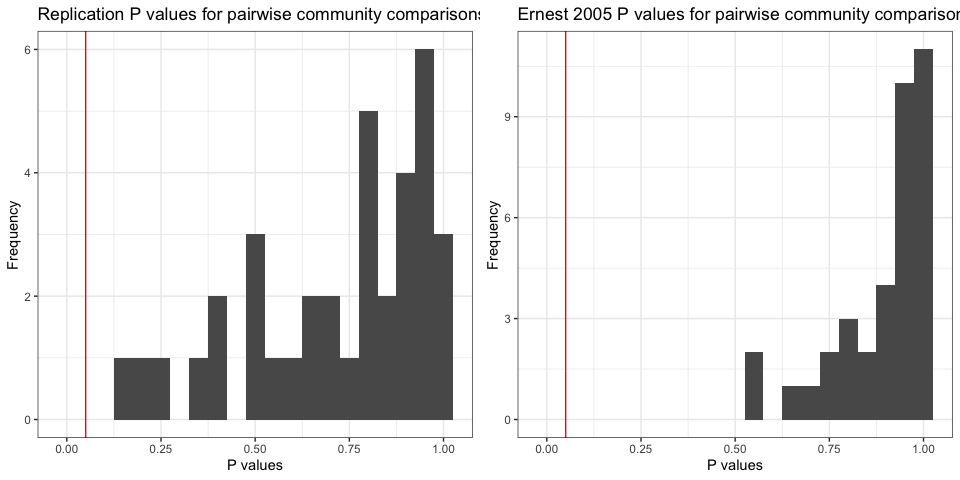
\includegraphics{ernest2005_replication_files/figure-latex/plot bsd crosscomm pval hist-1.pdf}


\end{document}
